\documentclass[a4paper,14pt]{scrartcl} 
\usepackage[utf8]{inputenc}
\usepackage[T1,T2A]{fontenc}
\usepackage[russian,english]{babel}
\usepackage{afterpage}
\usepackage{amsmath}
\usepackage{graphicx}
\usepackage{wrapfig}
\usepackage{setspace}
\doublespacing
\usepackage{pdfpages}
\addto\captionsenglish{\renewcommand\contentsname{Оглавление}}
\addto\captionsenglish{\renewcommand\figurename{Рис.}}


\begin{document}


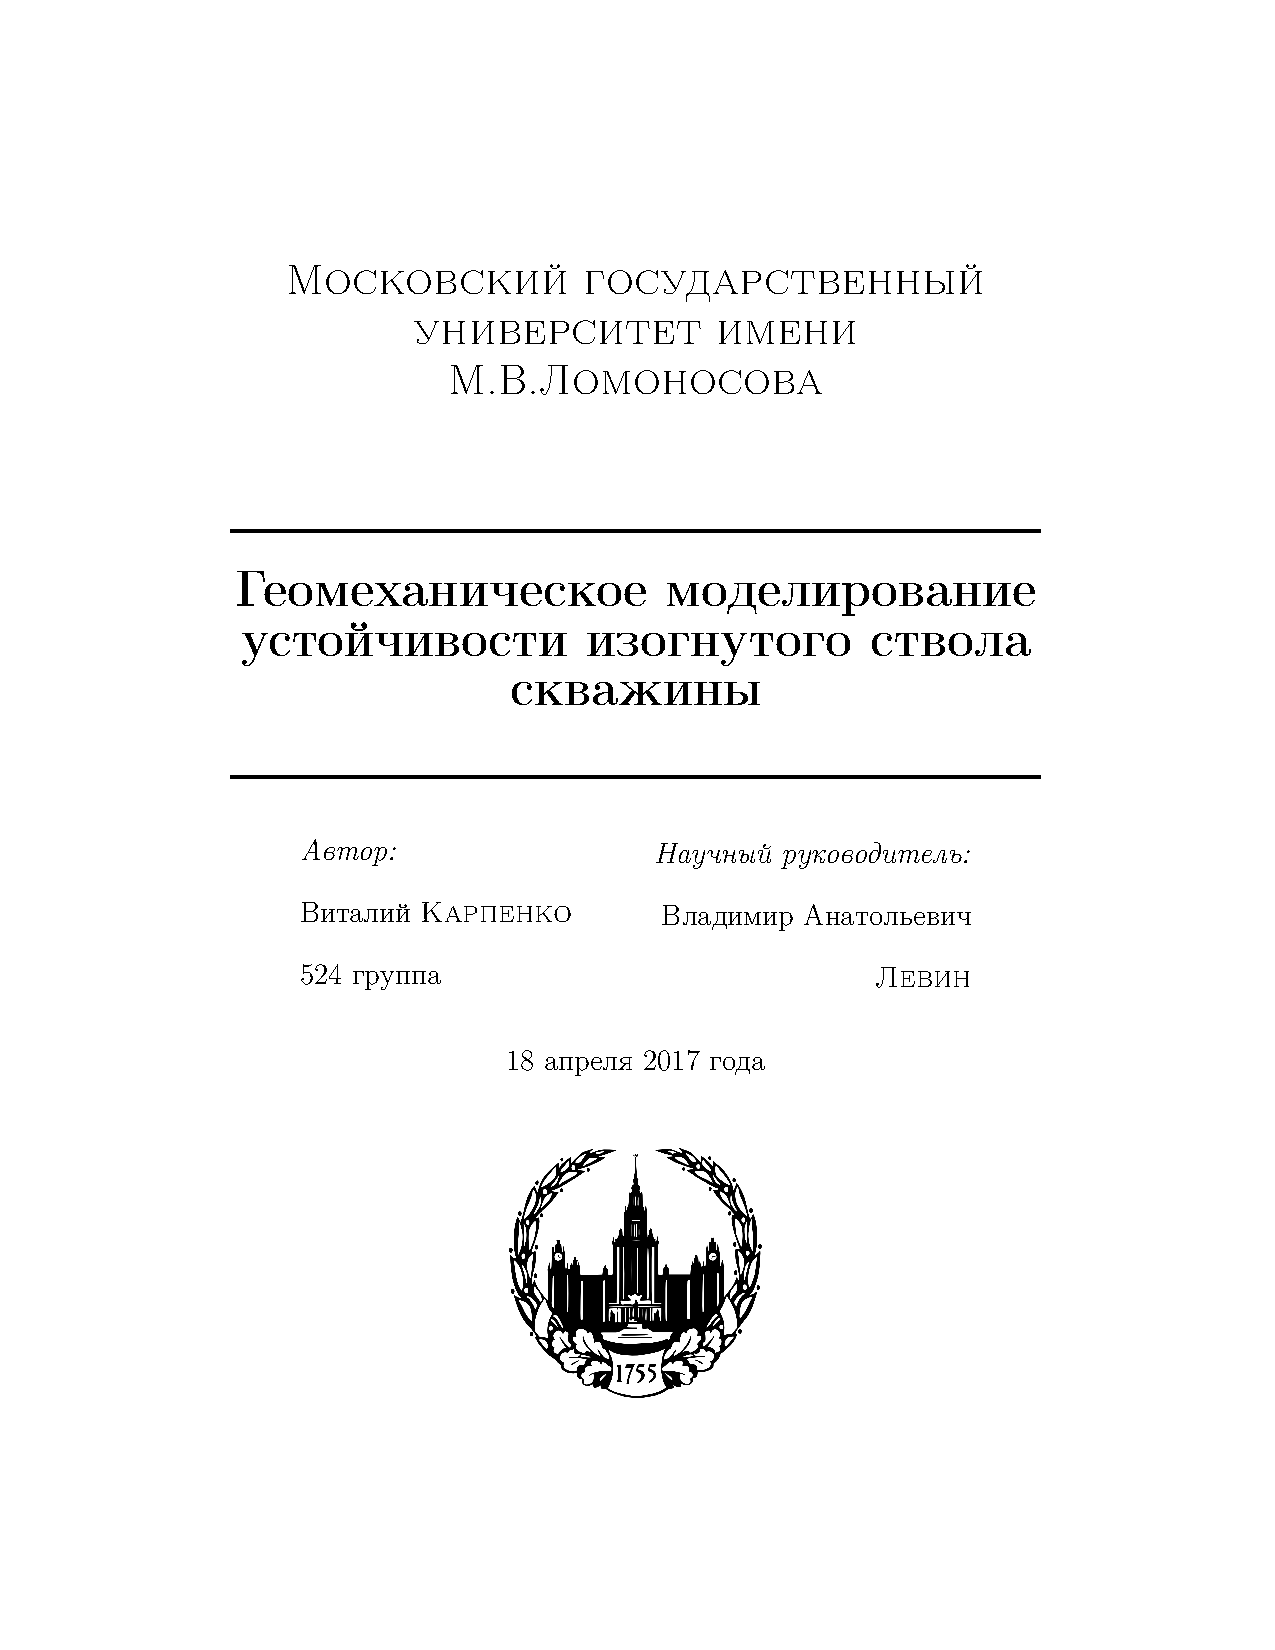
\includepdf[pages=1]{title.pdf}


\tableofcontents


\newpage
\section{Введение}
\subsection{О задаче}
Определение технологических параметров, при которых ствол скважины будет сохранять стабильное состояние – одна из важнейших задач геомеханики. Одним из параметров, которые могут относительно легко контроллироваться человеком и при этом оказывают значительное влияние на устойчивость (в каком смысле в данной работе употребляется этот термин будет пояснено далее), является плотность бурового раствора, который заливается в скважину во время бурения. Столб жидкости создаёт дополнительное давление в стволе, служащее "опорой", не позволяющей геометрии скважины уйти в область пластических деформаций под действием давления окружающих слоёв горных пород. 

\subsection{О работе}
В работе описывается разработка программы на языке Python, позволяющей по каротажным данным (т.е. информации о форме скважины, окружающих породах и т.д., полученной с помощью спуска-подъёма в скважине геофизического зонда) автоматически строить соответствующую им модель в препроцессоре CAE Fidesys и производить расчёт для определения оптимальной плотности бурового раствора - он должен быть достаточно плотным, чтобы удерживать ствол скважины от слишком сильных деформаций, но при этом не быть слишком плотным, чтобы не мешать процессу бурения.


\newpage
\section{Механическая постановка задачи}
\begin{itemize}
    \item Рассматривается изогнутая скважина круглого сечения (радиус может не быть константным).
    \item Деформации считаются малыми.
    \item Исследуется только область отстоящая от стенок скважины на расстояние $10r$, где $r$ - радиус скважины. Расположенные дальше горные породы нас не интересуют, т.к. к скважине прикладывается только давление столба жидкости, интеграл от которого по любому сечению, перпендикулярному направлению ствола, равен $0$ в силу симметрии. Следовательно, по принципу Сен-Венана, с удалением от концентратора напряжений (т.е. скважины) дополнительные напряжения, вызванные наличием скважины, будут затухать и на расстоянии на порядок превышающем характерный размер концентратора мы можем считать их пренебрежимо малыми.
    \item Материал упруго-пластический Друкера-Прагера.
    \item Свойства материала изменяются по оси OZ в соответствии с каротажными данными.
    \item Изнутри стенки скважины действует забойное давление.
\end{itemize}
\afterpage{%
\begin{wrapfigure}{R}{1\textwidth}
    \centering
    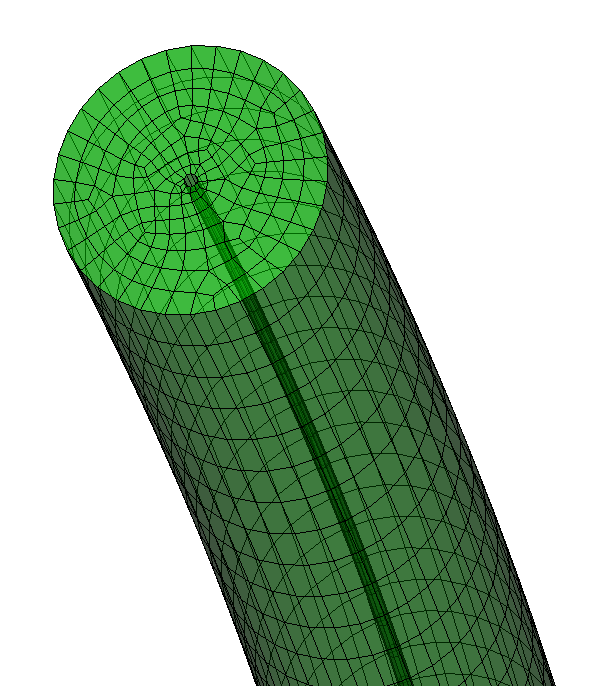
\includegraphics[width=1\textwidth]{images/well.png}
    \caption{\label{fig:well}Устье скважины.}
\end{wrapfigure}
\clearpage
}


\newpage
\section{Математическая постановка задачи}
\begin{enumerate}
    \item \blindtext
    \item \blindtext
\end{enumerate}


\end{document}
